
\chapter{Gráficos arboles binomiales}\label{anexograficos}

A continuación se incluyen diversos gráficos correspondientes al mismo árbol binomial de 10 pasos. Estos permiten observar la evolución de diferentes propiedades tales como la beta de la opción, el delta ($\Delta$) y el apalancamiento.

Los gráficos fueron realizados para una opción de compra con: precio inicial del subyacente = 100, precio de ejercicio = 105, tiempo = 1/2 año, volatilidad = 20\%, tasa libre de riesgo = 3\%, prima de riesgo del mercado ($\overline{r_M} - r_f$) es del 6\% y $\beta_S$ = 1.

\begin{figure}[H]
\centering
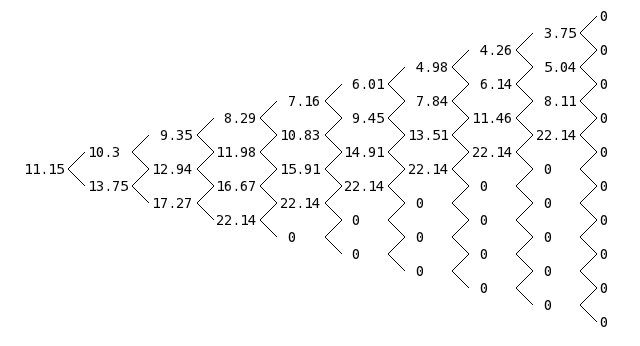
\includegraphics[width=1\textwidth]{Images/tree-betas.jpg}
\caption{Evolución de la $\beta$ de una opción en el árbol binomial de 10 pasos}
\label{fig:betaarbolchico}
\end{figure}

En la figura \ref{fig:deltaarbolchico} se ve la evolución del $\Delta$ (en rojo) con el cual se puede replicar una opción en un árbol binomial de 10 pasos. También se observa en azul el nivel de apalancamiento necesario para replicarla.

\begin{figure}[H]
\centering
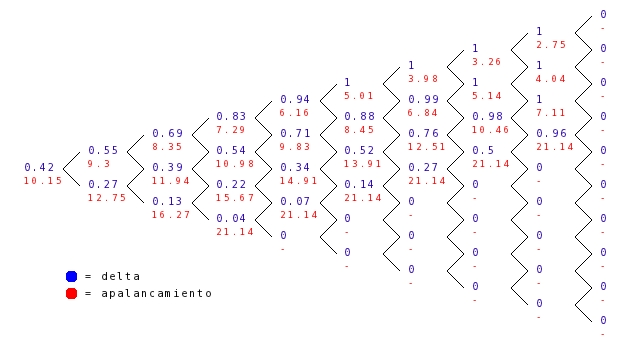
\includegraphics[width=1\textwidth]{Images/tree-delta-leverage.jpg}
\caption{Evolución del $\Delta$ y el apalancamiento en un árbol binomial de 10 pasos.}
\label{fig:deltaarbolchico}
\end{figure}

